% =============================================================================
% Pocket-sensitive somatic VEP -- final report
% Build:  make            (latexmk -> main.pdf)
% Clean:  make clean
%
% COURSE CONSTRAINTS:
%   - Main body: max 6 pages (3-4 ideal). References + appendices unlimited.
%   - Font: at least 11pt throughout (NeurIPS style hardcodes 10pt; switch
%     to article 11pt later if the grader enforces).
%
% PAGE BUDGET:
%   ~1.0 pg  Title + Background + Motivation
%   ~1.5 pg  Methods (pipeline, dataset, features, EDA, models)
%   ~1.5 pg  Results (macro-F1 + 1 sub-result)
%   ~1.0 pg  Discussion + Conclusion
%
% OWNERSHIP TAGS (grep these to find your work):
%   JR: = Johnathan to do
%   RW: = Ray to do (writing or plot)
% =============================================================================

\documentclass{article}

% neurips_2024.sty loads natbib internally; pass numeric-citation options
% in BEFORE the style file gets to it. `numbers` flips natbib to [n]
% citations, `sort&compress` collapses [1,2,3,5] into [1-3,5].
\PassOptionsToPackage{numbers,sort&compress}{natbib}

\usepackage[final]{neurips_2024}

% Replace the NeurIPS conference footer on the title page with our course
% attribution. Overrides \@noticestring from neurips_2024.sty so the
% vendored style file stays untouched.
\makeatletter
\renewcommand{\@noticestring}{%
  Artificial Intelligence in Genomics final project, Spring 2026, Nadav Brandes.%
}
\makeatother

\usepackage[utf8]{inputenc}
\usepackage[T1]{fontenc}
\usepackage{microtype}
\usepackage{graphicx}
\usepackage{booktabs}
\usepackage{float}
\usepackage{amsmath, amssymb}
\usepackage{siunitx}
\usepackage{xcolor}
\usepackage{hyperref}
\usepackage{url}
\usepackage{underscore}
% natbib is auto-loaded by neurips_2024.sty; do not load here.

% Figure captions: Helvetica (via helvet) and one step smaller than the
% body. Saves vertical space on figure-heavy pages and visually
% distinguishes captions from body prose. labelfont=bf keeps the
% "Figure N:" prefix bold so the caption start is still scannable.
\usepackage{helvet}
\usepackage{caption}
\captionsetup{font={sf,footnotesize}, labelfont={sf,bf,footnotesize},
               skip=4pt, belowskip=0pt}

% Tighten float spacing so [t]-placed figures can leak into the upper
% margin instead of sitting in default ~20pt of whitespace. Affects every
% \begin{figure} in the doc uniformly. Defaults are roughly 20pt for each
% of these; the values below pull figures closer to the surrounding text
% and to the page top edge.
\setlength{\textfloatsep}{6pt plus 2pt minus 2pt}  % between text and top/bottom floats
\setlength{\intextsep}{6pt plus 2pt minus 2pt}     % around in-text floats
\setlength{\floatsep}{8pt plus 2pt minus 2pt}      % between two floats on the same page
\setlength{\abovecaptionskip}{4pt}                  % between figure and its caption

\graphicspath{{figures/}}

\title{Pocket-sensitive somatic variant effect prediction (VEP)\\
  using AlphaFold-predicted protein structures}

\author{%
  Ray Wen \quad Johnathan Rafailov \\
  Courant Institute of Mathematical Sciences \\
  New York University \\
  \texttt{\{rw2604, rafaij01\}@nyu.edu}
}

\date{Artificial Intelligence in Genomics Final Project, Spring 2026}

\begin{document}
\maketitle

\begin{abstract}
Most missense variant effect predictors (VEPs) rely on sequence and
evolutionary conservation, with 3D structural context entering only
implicitly through learned representations. Driver variants are not spatially random. They cluster at functional
sites like binding pockets and modulatory sites, where a model that
sees a residue's spatial relationship to the pocket has access to
information that the residue-level sequence cannot recover. We test whether
explicit pocket-aware features carry signal beyond what sequence and
conservation already encode with a three-way orthogonal ablation across
sequence, structure (AlphaFold + \texttt{fpocket} + DSSP), and
evolution (phyloP100way, phastCons100way) feature blocks on 30{,}620
labeled ClinVar missense variants spanning 1{,}040 genes. Three
classifiers (random forest, MLP, XGBoost) are trained on each
single-modality arm, every pairwise combination, and the full union, swept
across five gene-grouped seeds. The union beats every constituent in
every model (macro F1 $0.85$--$0.86$ vs. best single-modality
$0.74$--$0.78$), and every pairwise combination also beats its best
constituent. Structural and evolutionary features carry information
that sequence-only features do not recover.
\end{abstract}

\section{Background}
\label{sec:background}

Cancer treatment regularly incorporates tumor sequencing and other biomarker
assays \citep{berger2018genomics, hadi2026gos} to identify disease-defining and actionable alterations among the thousands to
hundreds of thousands of somatic mutations a tumor can accumulate
\citep{kinnersley2024wgs}. OncoKB, an FDA-recognized\footnote{First somatic-variant knowledge base granted U.S. FDA partial recognition (October 2021); see the FDA list of recognized human genetic variant databases at \url{https://www.fda.gov/medical-devices/precision-medicine/fda-recognition-public-human-genetic-variant-databases}.} precision oncology knowledge base maintained
by Memorial Sloan Kettering Cancer Center and canonical source in the cancer genomics community \citep{chakravarty2017oncokb}, curates 155 somatic driver
% Counts from data/reference/oncokb_actionable_levels.tsv (pulled 2026-05-13):
% 155 unique (gene, alteration) pairs across 77 genes, matched to 157
% drugs across 75 cancer indications.
alterations across 77 genes that have matched targeted therapies
in routine clinical use\footnote{OncoKB Actionable Genes table (\url{https://www.oncokb.org/actionable-genes}), accessed 2026-05-13.}, including BRAF V600E in melanoma
(dabrafenib + trametinib), EGFR exon 19 deletions in NSCLC (osimertinib),
KRAS G12C in NSCLC and colorectal cancer (sotorasib, adagrasib), and HER2
amplification in breast and gastric cancers (trastuzumab and HER2-directed
ADCs). Targeted drugs made up 91\% of FDA oncology approvals
between 2000 and 2022 \citep{scott2023fdatrends}, and basket trials
increasingly enroll patients on the basis of a shared molecular feature
regardless of tumor origin \citep{bartoszkiewicz2026basket}, with programs
like KEYNOTE-158 \citep{marabelle2020keynote158} serving as a proof of concept for
tissue-agnostic FDA approvals. 

However, that 77-gene actionable set is a fraction of the broader
driver landscape. The rest is a long tail of less common variants, most
of which are not yet functionally characterized or therapeutically
actionable. \citet{kinnersley2024wgs} reported 74 driver genes new to
any cancer in their 100kGP cohort, with 88\% of those appearing at
frequencies below 10\% in their respective tumor types, and 79\% of
the 330 drivers in that cohort have no therapeutic target annotation
in COSMIC or OncoKB. The bottleneck for growing the actionable driver
catalog is variant interpretation, not data generation. Computational
variant effect prediction is the nomination step in that workflow, and
it is the focus of this paper.

Variant nomination tools have gone through several generations. Alignment-based scoring such as SIFT (2001) \citep{ng2001sift}
and PolyPhen-2 (2010) \citep{adzhubei2010polyphen2} gave way to
conservation-derived scores like phyloP (2010) \citep{pollard2010phylop},
phastCons (2005) \citep{siepel2005phastcons}, and GERP (2005) \citep{cooper2005gerp},
and to ensemble combiners like CADD (2014) \citep{kircher2014cadd} and REVEL
(2016) \citep{ioannidis2016revel}. A cancer-specific lineage including CHASM
(2009) \citep{carter2009chasm}, FATHMM-cancer (2013) \citep{shihab2013fathmm}, and
CanDrA (2013) \citep{mao2013candra} trained directly on somatic data. Deep
generative models on protein-family alignments came next, with EVE (2021)
\citep{frazer2021eve} building on EVmutation (2017) \citep{hopf2017evmutation}
and DeepSequence (2018) \citep{riesselman2018deepsequence}, and PopEVE
(2025) \citep{orenbuch2025popeve} extending the family by folding in
population frequency. Protein language models like ESM (2021, 2023)
\citep{rives2021esm, lin2022esm2} followed, learning sequence
statistics over broader protein universes without explicit family
alignment. Through all of this, explicit 3D context has been hard to
use systematically. Structure-aware predictors like SuSPect (2014)
\citep{yates2014suspect} and the 3D hotspot analyses of
\citet{gao20173dhotspots} (2017) existed but were limited by patchy
experimentally resolved structures.

AlphaFold (2021, 2022) \citep{jumper2021alphafold, varadi2022alphafolddb} mitigated
this constraint by providing high-confidence predicted structures for
nearly the entire human proteome, and pocket-detection tools like
\texttt{fpocket} (2009) \citep{leguilloux2009fpocket} and P2Rank (2018)
\citep{krivak2018p2rank} could now run on any protein. The current
generation of VEPs has folded structural information into the modeling
pipeline, though almost always implicitly. AlphaMissense (2023)
\citep{cheng2023alphamissense} adapts an AlphaFold-style
sequence-to-structure architecture and trains on weak labels derived
from population allele frequency, PrimateAI-3D (2023)
\citep{gao2023primateai3d} uses a 3D convolution over predicted
neighborhoods, and ESM-family language models (2021) \citep{meier2021esm1v}
pick up structural regularities through pretraining without explicit
structural input. Because these models report a single combined score, it is hard to
tell which signal class is doing the work, and so it stays unclear
whether explicit pocket-level features add anything implicit
structural reasoning does not already capture.

We address that question with a controlled feature ablation on somatic
missense variants labeled as oncogenic or benign, featurizing each
variant along three orthogonal blocks (sequence, structure, and
evolution) and comparing every single-modality arm, every pairwise
combination, and the union under a gene-grouped train/val/test split
repeated across five seeds. This is a diagnostic ablation, not a new
state-of-the-art predictor, and we do not benchmark against
AlphaMissense. The question is whether explicit pocket conformation
carries information that current implicit structural reasoning
misses.

\begin{figure}[!t]
  \centering
  \makebox[\textwidth][c]{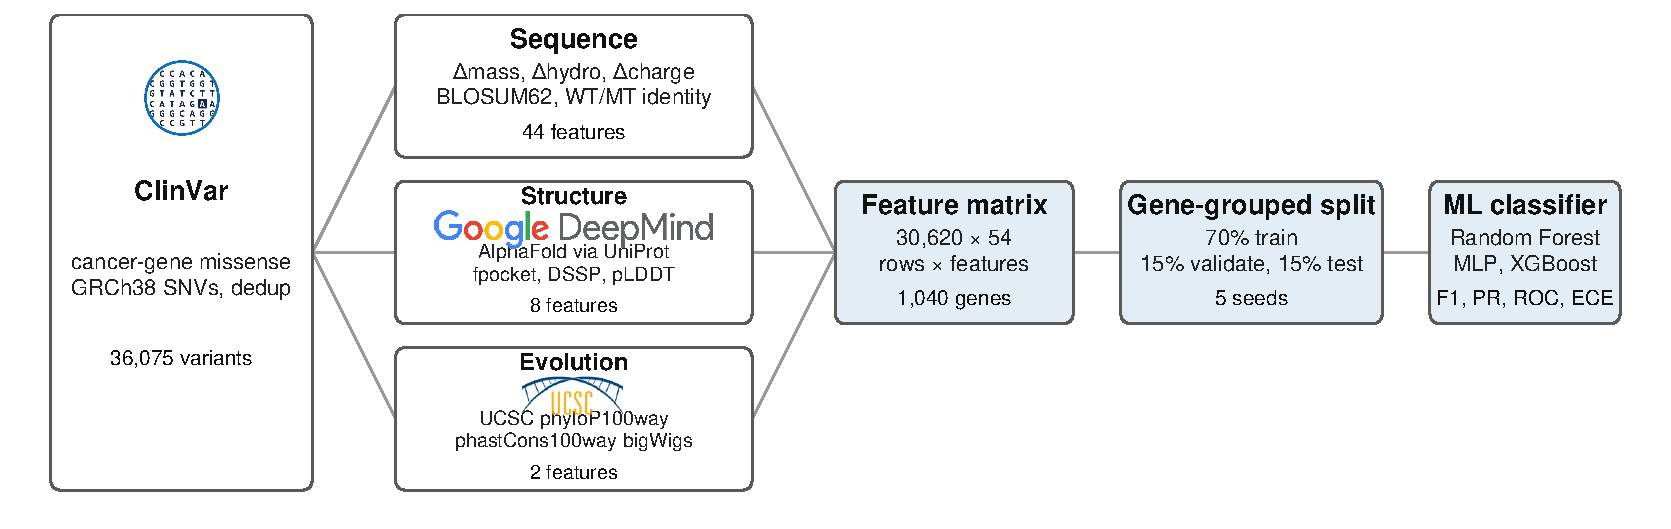
\includegraphics[width=1.2\linewidth]{pipeline.pdf}}
  \caption{End-to-end pipeline. Variant labels are resourced from ClinVar and
  bridged to AlphaFold structures via UniProt; sequence, structure
  (\texttt{fpocket} + \texttt{mkdssp} + pLDDT), and evolutionary
  (phyloP / phastCons) feature blocks are joined into a single feature
  matrix, then evaluated under a gene-grouped split.}
  \label{fig:pipeline}
\end{figure}

\section{Motivations \& Hypotheses}
\label{sec:motivation}

Driver variants are not spatially random. They cluster at residues
that regulate enzymatic activity, occupy interface positions, or sit
inside binding pockets that are themselves under selective pressure to
remain conserved. A model that sees a residue's pocket membership,
distance to the nearest pocket, and the druggability score of that
pocket has access to information a residue-only sequence model cannot
reconstruct without implicitly redoing structure prediction. The
ablation in this paper tests whether that information is recoverable
in practice and whether it adds to sequence and evolutionary
conservation rather than overlapping with them. We expect structure
features on their own to carry classification signal above the
prevalence baseline, every pairwise combination of sequence,
structure, and evolution to beat its better constituent modality, and
the union of all three to beat every pairwise combination.

\section{Methods}
\label{sec:methods}

\subsection{Dataset}
In the proposal we wanted to use OncoKB, which is the gold standard
for querying cancer pathogenicity and drugability labels. On review, their terms
of use bar reusing oncogenicity annotations as training labels for
machine learning models in both academic and commercial settings. We
instead resorted to ClinVar, which is not as curated. Its
\texttt{variant\_summary} dump is fully public and carries no such
restriction, and it has both an explicit oncogenicity column (449
variants in our final set) and a broader clinical-significance column
that we gated to OncoKB-curated cancer genes (gene names only, not
labels) to avoid pulling in hereditary-disease variants. The
oncogenicity-sourced rows drop from 449 to 434 after the inner join
against feature coverage. The raw dump has $\sim$8.9M rows; after
restricting to GRCh38 single-nucleotide missense substitutions and
collapsing codon-degenerate duplicates at the (\texttt{GeneSymbol},
\texttt{protein\_change}) level, we kept 36{,}075 labeled rows
spanning 1{,}073 genes \citep{landrum2018clinvar}.

For structural context we used the AlphaFold human proteome
(20{,}504 monomer PDB files, v4) \citep{jumper2021alphafold,
varadi2022alphafolddb}. ClinVar gene symbols were mapped to UniProt
accessions through UniProt's mapping service, yielding 16{,}620 unique
canonical accessions. Per-residue structural features were computed from
each predicted structure with \texttt{fpocket}
\citep{leguilloux2009fpocket} and \texttt{mkdssp}
\citep{kabsch1983dssp}.

For evolutionary context we used the UCSC \texttt{phyloP100way} and
\texttt{phastCons100way} bigWig tracks, which score nucleotide-level
conservation across a 100-vertebrate multiple alignment
\citep{pollard2010phylop, siepel2005phastcons}. The proposal originally
specified ConSurf-DB; we switched to phyloP/phastCons because they are
the canonical evolutionary signal used by REVEL, CADD, and dbNSFP, and
because ClinVar already provides the GRCh38 locus and so the join is direct
and per-nucleotide. ConSurf-DB remains available as a structure-aligned
follow-up signal.

The full feature matrix is built by inner-joining all three feature
blocks to the labeled set on a per-variant key, yielding 30{,}620 rows
across 1{,}040 genes with full feature coverage and a 1.47:1
benign:oncogenic ratio.

\subsection{Feature Engineering}
Features split into three orthogonal blocks. The \emph{sequence} block
holds per-substitution physicochemical deltas (mass, Kyte--Doolittle
hydropathy, net charge at pH~7), the BLOSUM62 substitution score, and
one-hot encodings of the WT and MT amino acid identities. The
\emph{structure} block holds \texttt{fpocket}-derived pocket geometry
(distance to nearest pocket, in-pocket flag, druggability),
\texttt{mkdssp}-derived solvent-accessible surface area and a 3-state
secondary-structure encoding, and the AlphaFold per-residue confidence
(pLDDT); pLDDT lives here rather than under sequence because it is a
structural-quality signal, and treating it as sequence-level would
muddy the orthogonality of the ablation. The \emph{evolution} block
holds UCSC phyloP100way and phastCons100way queried at the variant
nucleotide. Per-column definitions and sources are in Appendix B.

\subsection{Data Exploration}

\begin{figure}[t]
  \centering
  \makebox[\textwidth][c]{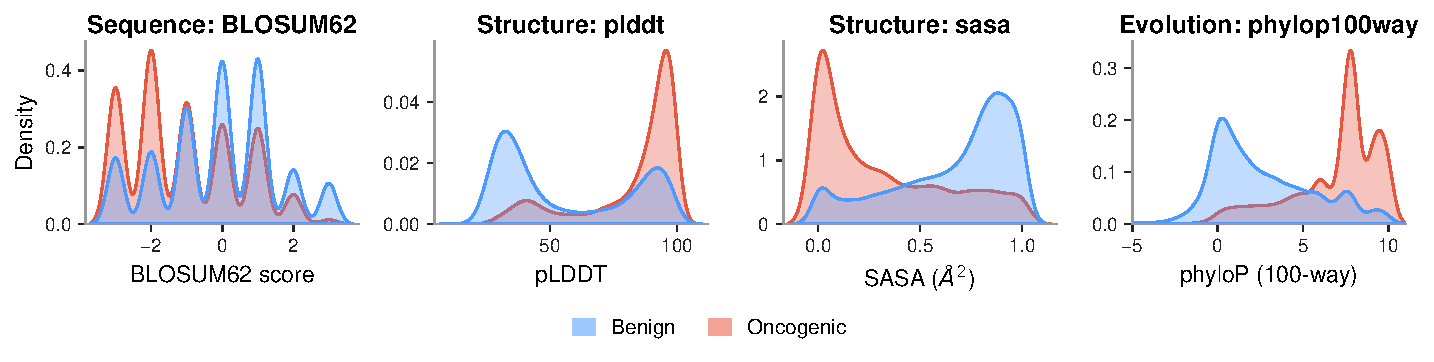
\includegraphics[width=1.2\linewidth]{numeric_distributions_report.pdf}}
  \caption{Per-feature distributions across the three feature blocks
  (sequence, structure, evolution), split by oncogenicity label. Kernel
  density estimates with class-wise normalization.}
  \label{fig:distributions}
\end{figure}

Figure~\ref{fig:distributions} shows a subset of features from all
three blocks (sequence, structure, evolution). BLOSUM62 separates the
two classes somewhat, with oncogenic variants skewing negative and
benign variants skewing positive or zero, though the two distributions
still overlap. The structure and evolution features separate the
classes more cleanly. pLDDT and SASA (solvent-accessible surface area)
both show visibly different peaks between benign and oncogenic
variants, and \texttt{phyloP100way} behaves similarly. On these
distributions alone the structure and evolution blocks look like the
stronger candidates going into the model.

\subsection{Model Choice \& Evaluation}
We evaluate three model families spanning bagged trees, boosted trees,
and a small neural network, and so the ablation isolates the effect of the
feature blocks rather than any single inductive bias. For the random
forest we use sklearn's \texttt{RandomForestClassifier} with
\texttt{n\_estimators=300}, unbounded depth, \texttt{min\_samples\_leaf=2},
and \texttt{class\_weight="balanced"} \citep{pedregosa2011sklearn}. For
the MLP we use sklearn's \texttt{MLPClassifier} wrapped in a
\texttt{StandardScaler} then \texttt{MLP} pipeline (since the input columns mix
0/1 binary columns, pLDDT in $[0, 100]$, and unbounded floats); the MLP has
two hidden layers of size 32 and 16, \texttt{max\_iter=1000}, and
\texttt{early\_stopping=True} with \texttt{n\_iter\_no\_change=20}
\citep{pedregosa2011sklearn}. For XGBoost we use \texttt{XGBClassifier}
with \texttt{n\_estimators=300}, \texttt{max\_depth=4}, learning rate
$0.1$, log-loss eval metric, and \texttt{scale\_pos\_weight} set per
split to the empirical $n_{\text{neg}} / n_{\text{pos}}$ ratio of the
training fold ($\approx 1.47$) \citep{chen2016xgboost}.

\subsection{Class Distribution and Splits}
The labels are mildly imbalanced at $\approx$1.47:1 benign:oncogenic.
The random forest is calibrated for this this through
\texttt{class\_weight="balanced"} and XGBoost through
\texttt{scale\_pos\_weight} set per split to the training-fold
$n_{\text{neg}} / n_{\text{pos}}$. sklearn's MLP has no
\texttt{class\_weight} parameter and we fit it unweighted; this leaves
the MLP at a small disadvantage on the most imbalanced single-modality
arms (visible as the larger gap between MLP and tree-based models on
the sequence-only setting) but does not affect the ablation
conclusion, which is driven by feature-set deltas an order of magnitude
larger than the model-vs-model spread.

Splits are gene-grouped (sklearn \texttt{GroupShuffleSplit} on
\texttt{GeneSymbol}) at 70 / 15 / 15 train / val / test; this is so that no protein
reappears in both training and test evaluation. This is critical here
because variants within a single oncogene tend to share a label, and
without grouping the model can learn a gene-identity shortcut that
inflates test metrics beyond what the features actually provide. Each of
the five seeds redraws the gene partition and refits the models;
per-split label balance is printed at runtime and so, any drift from the
overall 1.47:1 ratio is visible.

\section{Results}
\label{sec:results}

A full table of the results for the 7 feature set combinations and 3 models
can be found in the Appendix (Table~\ref{tab:full-results}).

% Top: macro-F1 bars per (config, classifier) from
% scripts/visualize_results.py (headline_macro_f1_perconfig). Bottom:
% test-set ROC curves from scripts/plot_roc_curves.py (seed=42, one
% panel per classifier). Bars and curves share a per-config palette so
% each feature configuration tracks visually from the bar above to the
% line below within the same classifier column.
\begin{figure}[t]
  \centering
  \makebox[\textwidth][c]{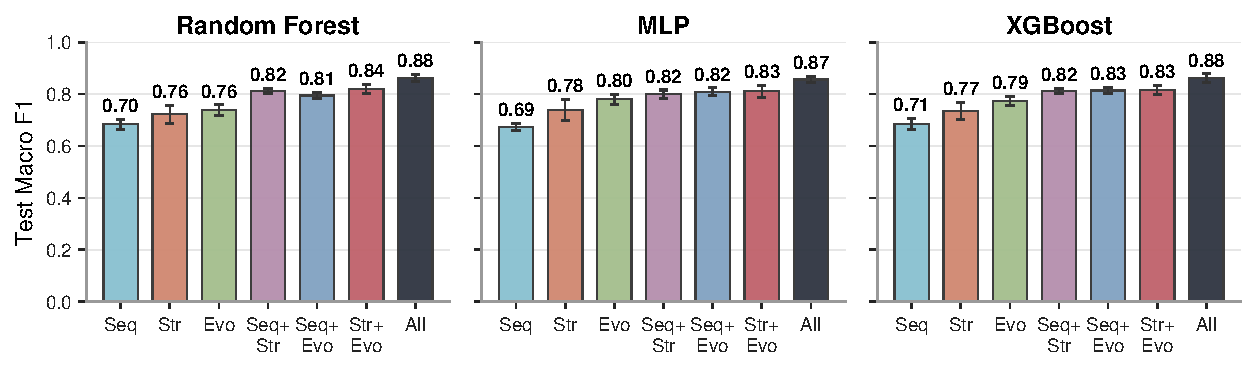
\includegraphics[width=1.2\linewidth]{headline_macro_f1_perconfig.pdf}}\\[0.6em]
  \makebox[\textwidth][c]{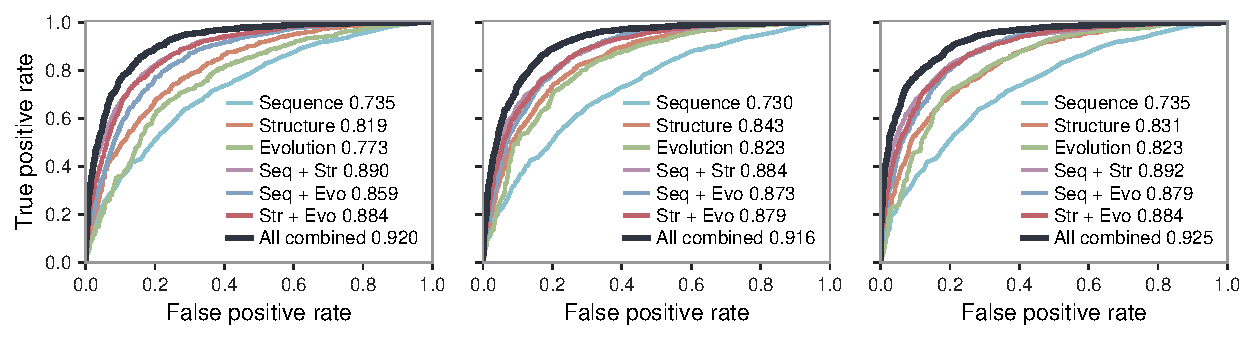
\includegraphics[width=1.2\linewidth]{roc_curves_per_model.pdf}}
  \caption{\textbf{(Top)} Test macro-F1 across the seven feature
  configurations, faceted by classifier. Error bars span $\pm 1$ std
  over 5 gene-grouped seeds. \textbf{(Bottom)} Test-set ROC curves for
  the same seven configurations, with one panel per
  classifier. Bars and curves use a shared color palette so
  the same color traces a feature set from its macro-F1 bar to its
  ROC curve directly below.}
  \label{fig:headline}
\end{figure}

\subsection{Relative Model Performance}
The full union of sequence, structure, and evolutionary features
achieves the best macro-F1 in every model (Random Forest
$0.863\pm0.013$, MLP $0.857\pm0.013$, XGBoost $0.861\pm0.018$ on test)
and dominates every single-modality and pairwise arm. Among
single-modality arms the ordering is consistent, with evolution
beating structure beating sequence and a spread of $\approx 0.10$
macro-F1 from worst to best ($0.68$ for sequence, $0.74$ for
structure, $0.78$ for evolution). The seed-to-seed standard deviation also
shrinks monotonically with feature richness, from $\sigma\approx 0.03$
on the structure-only arm to $\sigma\approx 0.014$ on the union, so
richer feature sets yield more stable training as well as higher mean
performance. Beyond raw macro-F1, every pairwise combination beats
its strongest single-modality constituent ($+0.03$ to $+0.09$
macro-F1) and the union beats its strongest single ($+0.08$ to
$+0.12$). No one modality is carrying the headline number with
the others contributing noise. This matches what we expected for
structure features carrying signal on their own and for the union
beating every pairwise combination.

\section{Discussion}
\label{sec:discussion}

% Rendered by scripts/visualize_case_study.py from
% data/raw/alphafold/AF-P00519-F1-model_v4.pdb.gz and the pocket residues
% in data/processed/structure_features.parquet. ABL1 A433T is a test-set
% variant the all-features XGBoost rescued (p_seq=0.22, p_all=0.89).
\begin{figure}[t]
  \centering
  \makebox[\textwidth][c]{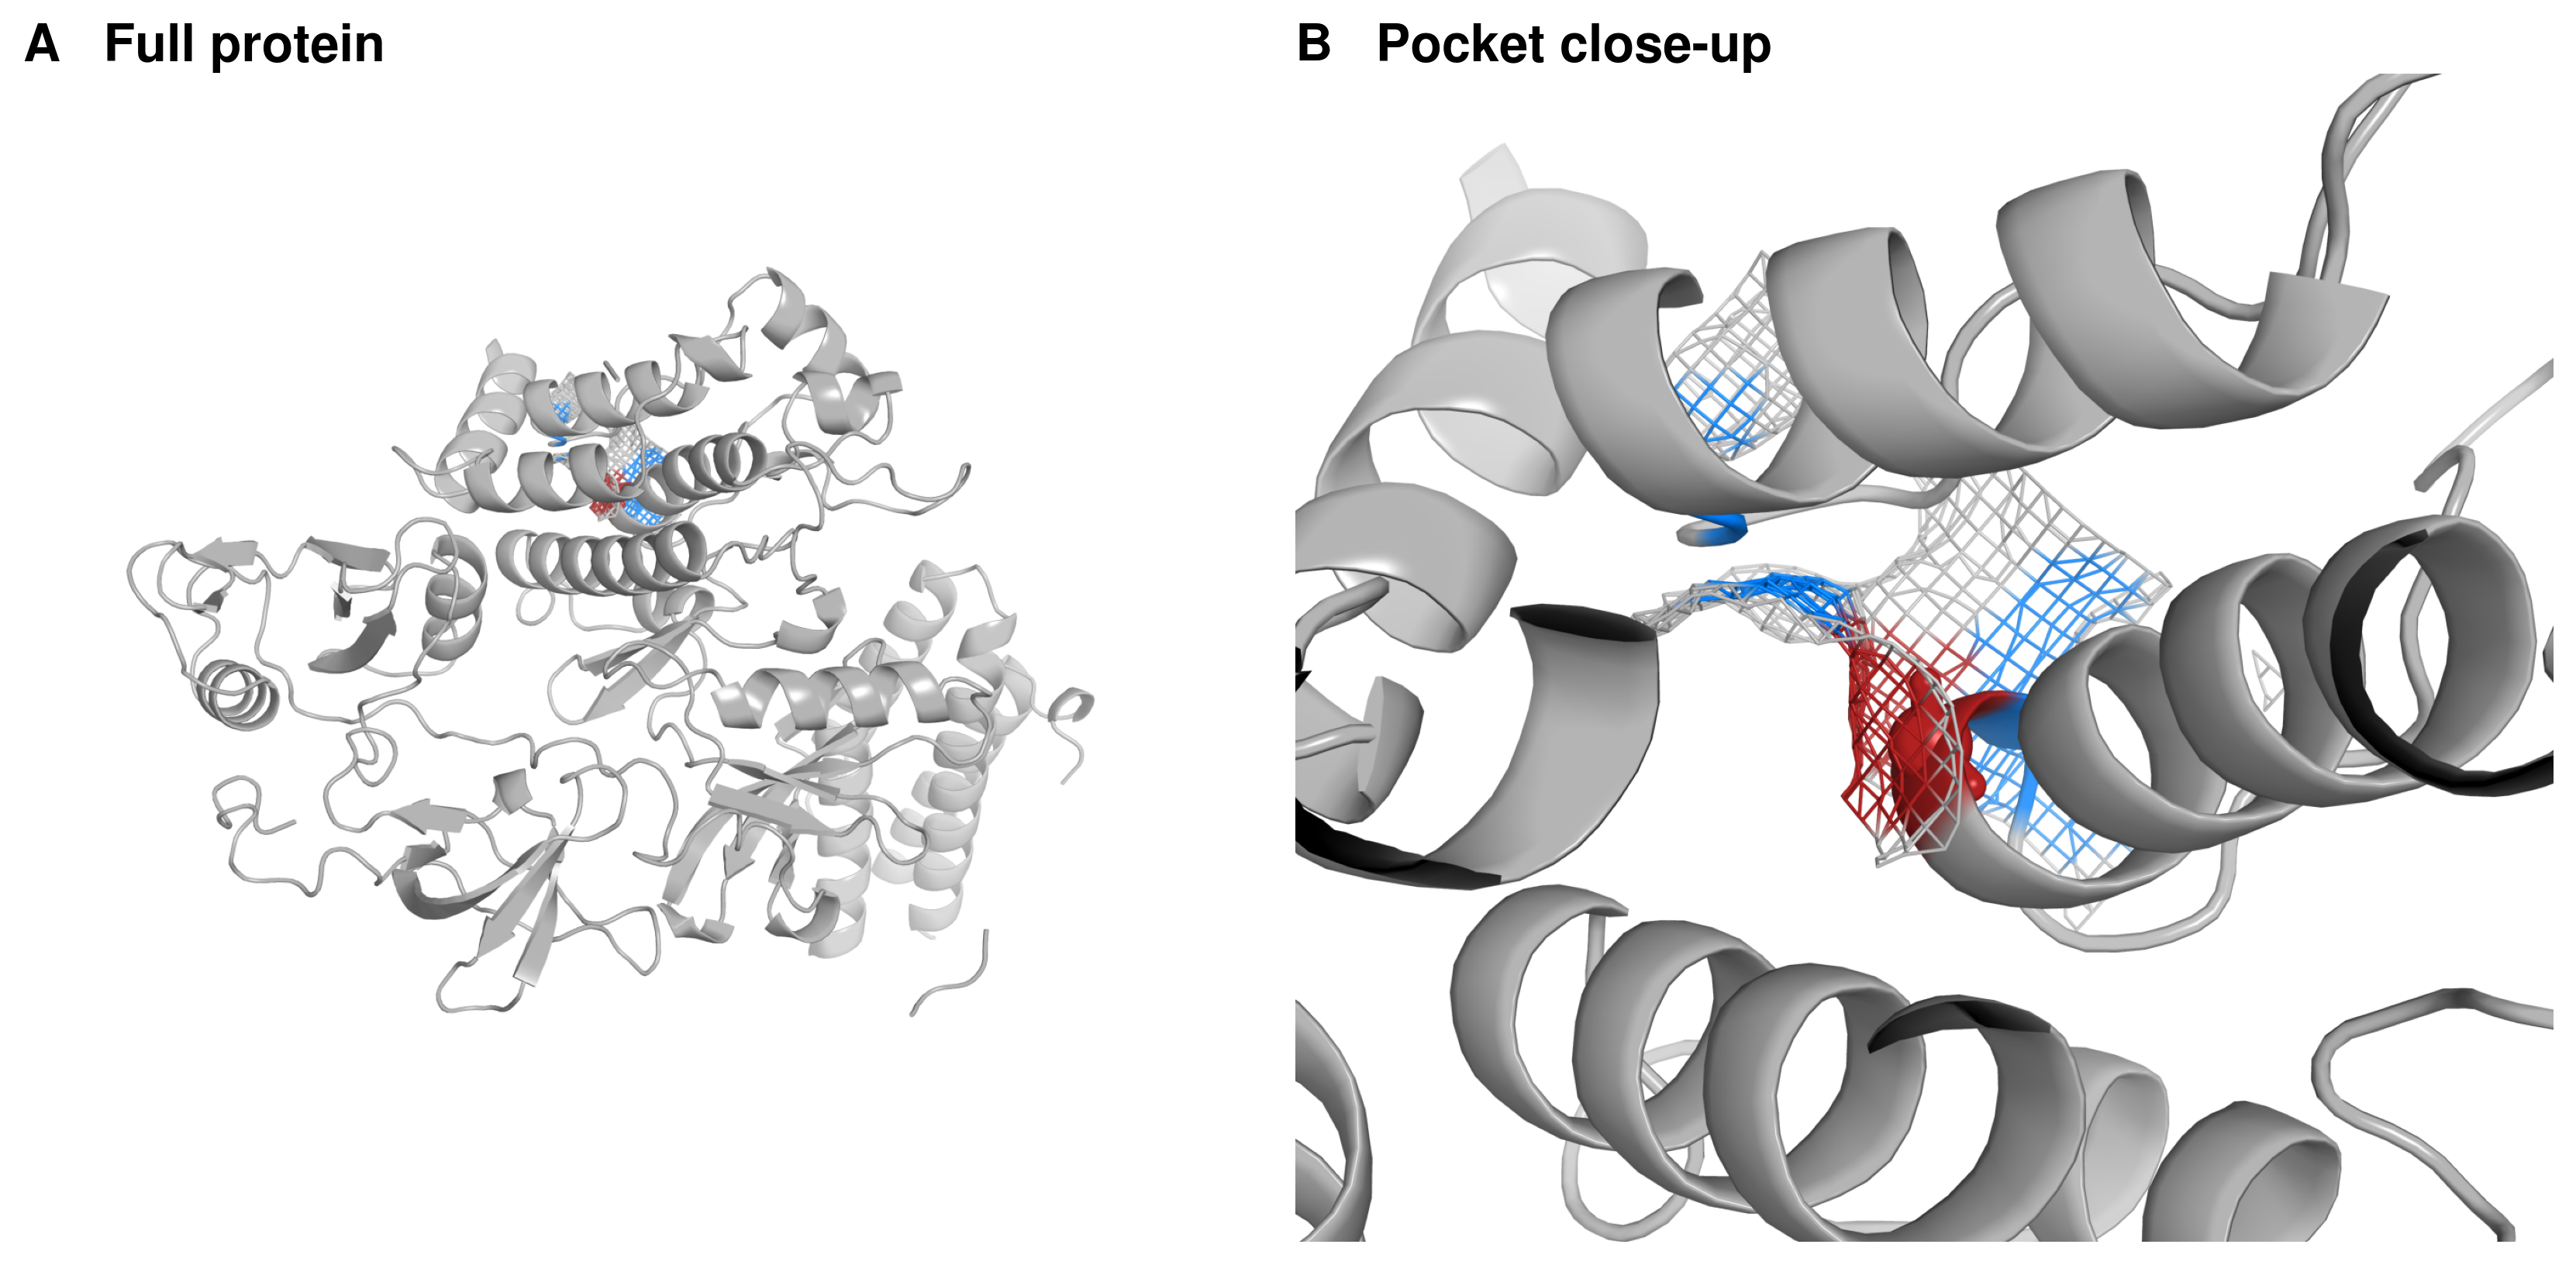
\includegraphics[width=1.10\linewidth]{case_study.png}}
  \caption{Case study, ABL1 p.A433T. \textbf{(A)} The variant
  residue (red) located within the AlphaFold-predicted ABL1 kinase
  fold; disordered tails (pLDDT $<50$) are hidden for clarity.
  \textbf{(B)} A closeup of the residue inside its
  \texttt{fpocket}-predicted binding pocket (light-blue mesh), with
  pocket-lining residues drawn as blue sticks. On the test
  set the sequence-only XGBoost called this variant benign
  ($p = 0.22$); the full-feature model recovered the correct oncogenic
  call ($p = 0.89$). The sequence change A>T is modest on
  conventional substitution scores, but the structural context
  (deeply buried inside a druggable pocket, pLDDT $0.98$) and high
  evolutionary conservation (phyloP $10.0$) cause it to be flagged.}
  \label{fig:case-study}
\end{figure}

Permutation importance on the union arm agrees across all three
models on which features are contributing most.
The top four features by importance are, in order,
\texttt{phylop100way}, \texttt{plddt}, \texttt{sasa}, and
\texttt{BLOSUM62}; \texttt{phastcons100way} and the pocket features
sit in the next tier. The strongest single feature is evolutionary
conservation (consistent with the broader missense-VEP literature), but
the second- and third-strongest are both structural, and crucially
neither of them comes from \texttt{fpocket}. \texttt{plddt} is
AlphaFold's per-residue confidence, and \texttt{sasa} is the
DSSP-derived solvent exposure of the residue. Both encode information
about how exposed and well-modeled the residue is, and neither is
recoverable from sequence alone. The explicit pocket-geometry features
(\texttt{dist\_to\_nearest\_pocket}, \texttt{druggability},
\texttt{in\_pocket}) carry smaller individual importances but still
contribute on top of pLDDT and SASA, which is why the structure-only
arm reaches $0.74$ macro-F1 rather than the $0.68$ ceiling of
sequence-only. The union's win over single-modality arms is not driven by any one
feature. It comes from combining three moderately strong signals from
different sources.

A second pattern in the headline table is that the gap between models
shrinks as the feature set grows, which says the wins are feature-driven
rather than model-driven. In all
three models, the union of all feature sets yields a consistent
$+0.17$--$0.18$ macro-F1 improvement, while the difference between
models on the same feature set is less than $0.006$ for the combined
set and less than $0.019$ for the individual feature sets, both of
which fall within seed-to-seed noise. Model choice only mattered for
the sequence-only feature set, where MLP underperformed tree-based
models by about $0.01$ macro-F1, suggesting that tree models are more robust
when the feature set is thin.

Figure~\ref{fig:case-study} shows what this looks like for a single
variant. ABL1 is a non-receptor tyrosine kinase whose BCR-ABL fusion
drives chronic myeloid leukemia and is the canonical target of
imatinib, the first kinase inhibitor approved in oncology. Position
433 sits in the kinase domain, where the ATP-binding pocket is both
catalytically essential and a known drug-binding site. ABL1 p.A433T
is a variant in the test set that the sequence-only XGBoost called benign
($p = 0.22$) and the full-feature model rescued to a correct oncogenic
call ($p = 0.89$). On BLOSUM62 alone the A to T swap is mild and so a
model with nothing else to look at has no real reason to flag it. The full-feature model observes something different.
The residue sits deep inside a druggable pocket (panel B), AlphaFold
  is confident in that placement (pLDDT $0.98$), and the position is among most conserved (phyloP $10.0$). Sequence said benign and structure plus evolution
said oncogenic, and the latter is correct. One example does
not generalize, but it shows the mechanism the headline numbers are
picking up.

\section{Conclusion}
\label{sec:conclusion}

A three-way orthogonal ablation across sequence, structure, and
evolutionary feature blocks shows that each modality carries
non-redundant predictive signal for classifying missense variants as
oncogenic versus benign. The full union beats every single-modality and
pairwise arm in all three model classes, and every multi-modal
combination beats the best of its constituents. Pocket-aware structural
features are informative both on their own and inside the union, which
supports the hypothesis that 3D context adds signal beyond what
sequence- and conservation-based predictors already capture. Natural next steps include benchmarking against
AlphaMissense as an explicit upper bound, replacing \texttt{fpocket}
with P2Rank for pocket detection, and extending the feature block to
include structural-aligned conservation (e.g.\ ConSurf-DB) on top of
the per-base phyloP/phastCons signal.

\clearpage
\appendix

\noindent{\large\bfseries Appendix A: Full results table}\par
\vspace{0.4em}
\label{app:full-results}

\begin{table}[H]
  \centering
  \caption{Test split, mean $\pm$ std across 5 seeds. Bold = best feature
  set within each model (per metric); lower = better for ECE.}
  \label{tab:full-results}
  \footnotesize
  \setlength{\tabcolsep}{4pt}
  \makebox[\textwidth][c]{%
  \begin{tabular}{llccccc}
    \toprule
    Feature set & Model & Macro F1 & PR-AUC & ROC-AUC & Bal.\ Acc. & ECE \\
    \midrule
    Sequence     & Random Forest & $0.684 \pm 0.018$ & $0.654 \pm 0.041$ & $0.747 \pm 0.018$ & $0.688 \pm 0.020$ & $0.074 \pm 0.013$ \\
    Sequence     & MLP           & $0.674 \pm 0.015$ & $0.654 \pm 0.041$ & $0.746 \pm 0.018$ & $0.670 \pm 0.015$ & $0.030 \pm 0.006$ \\
    Sequence     & XGBoost       & $0.686 \pm 0.021$ & $0.655 \pm 0.041$ & $0.748 \pm 0.018$ & $0.690 \pm 0.021$ & $0.075 \pm 0.014$ \\
    \midrule
    Structure    & Random Forest & $0.723 \pm 0.034$ & $0.718 \pm 0.028$ & $0.806 \pm 0.037$ & $0.721 \pm 0.035$ & $0.045 \pm 0.028$ \\
    Structure    & MLP           & $0.740 \pm 0.040$ & $0.737 \pm 0.034$ & $0.818 \pm 0.045$ & $0.741 \pm 0.043$ & $0.050 \pm 0.013$ \\
    Structure    & XGBoost       & $0.736 \pm 0.032$ & $0.731 \pm 0.028$ & $0.819 \pm 0.036$ & $0.740 \pm 0.037$ & $0.062 \pm 0.014$ \\
    \midrule
    Evolution    & Random Forest & $0.739 \pm 0.020$ & $0.700 \pm 0.026$ & $0.804 \pm 0.022$ & $0.740 \pm 0.021$ & $0.105 \pm 0.014$ \\
    Evolution    & MLP           & $0.780 \pm 0.019$ & $0.761 \pm 0.029$ & $0.848 \pm 0.017$ & $0.781 \pm 0.019$ & $0.037 \pm 0.005$ \\
    Evolution    & XGBoost       & $0.774 \pm 0.017$ & $0.774 \pm 0.036$ & $0.853 \pm 0.019$ & $0.779 \pm 0.017$ & $0.066 \pm 0.005$ \\
    \midrule
    Seq + Struct & Random Forest & $0.813 \pm 0.008$ & $0.853 \pm 0.011$ & $0.895 \pm 0.009$ & $0.814 \pm 0.008$ & $0.027 \pm 0.005$ \\
    Seq + Struct & MLP           & $0.800 \pm 0.016$ & $0.841 \pm 0.013$ & $0.888 \pm 0.011$ & $0.799 \pm 0.018$ & $0.031 \pm 0.011$ \\
    Seq + Struct & XGBoost       & $0.812 \pm 0.009$ & $0.856 \pm 0.009$ & $0.897 \pm 0.009$ & $0.817 \pm 0.009$ & $0.041 \pm 0.013$ \\
    \midrule
    Seq + Evo    & Random Forest & $0.795 \pm 0.012$ & $0.817 \pm 0.028$ & $0.880 \pm 0.013$ & $0.798 \pm 0.012$ & $0.059 \pm 0.010$ \\
    Seq + Evo    & MLP           & $0.809 \pm 0.016$ & $0.831 \pm 0.025$ & $0.894 \pm 0.014$ & $0.813 \pm 0.017$ & $0.023 \pm 0.007$ \\
    Seq + Evo    & XGBoost       & $0.814 \pm 0.013$ & $0.847 \pm 0.025$ & $0.900 \pm 0.013$ & $0.823 \pm 0.014$ & $0.050 \pm 0.007$ \\
    \midrule
    Struct + Evo & Random Forest & $0.819 \pm 0.017$ & $0.840 \pm 0.022$ & $0.899 \pm 0.016$ & $0.820 \pm 0.017$ & $\mathbf{0.022 \pm 0.004}$ \\
    Struct + Evo & MLP           & $0.811 \pm 0.022$ & $0.831 \pm 0.024$ & $0.892 \pm 0.020$ & $0.813 \pm 0.021$ & $0.028 \pm 0.010$ \\
    Struct + Evo & XGBoost       & $0.815 \pm 0.018$ & $0.845 \pm 0.019$ & $0.900 \pm 0.015$ & $0.822 \pm 0.018$ & $0.043 \pm 0.014$ \\
    \midrule
    All Combined & Random Forest & $\mathbf{0.863 \pm 0.013}$ & $\mathbf{0.901 \pm 0.016}$ & $\mathbf{0.936 \pm 0.010}$ & $\mathbf{0.866 \pm 0.011}$ & $0.030 \pm 0.004$ \\
    All Combined & MLP           & $\mathbf{0.857 \pm 0.013}$ & $\mathbf{0.889 \pm 0.017}$ & $\mathbf{0.930 \pm 0.012}$ & $\mathbf{0.859 \pm 0.011}$ & $\mathbf{0.020 \pm 0.006}$ \\
    All Combined & XGBoost       & $\mathbf{0.861 \pm 0.018}$ & $\mathbf{0.908 \pm 0.011}$ & $\mathbf{0.939 \pm 0.009}$ & $\mathbf{0.867 \pm 0.016}$ & $\mathbf{0.034 \pm 0.013}$ \\
    \bottomrule
  \end{tabular}%
  }
\end{table}

\clearpage
\noindent{\large\bfseries Appendix B: Full feature listing}\par
\vspace{0.4em}
\label{app:features}

The feature matrix has 54 columns across three orthogonal blocks
(Table~\ref{tab:features}). The \texttt{sequence} block is purely a
function of the wild-type and mutant residue identities and their
physicochemical deltas; the \texttt{structure} block is per-residue
output from AlphaFold + \texttt{fpocket} + \texttt{mkdssp}; the
\texttt{evolution} block is per-nucleotide UCSC phyloP and phastCons.

\begin{table}[H]
  \centering
  \caption{Per-column feature listing. AA binary-column flags are collapsed onto
  single rows (the 20 canonical amino acids). Block totals: sequence
  = 44, structure = 8, evolution = 2.}
  \label{tab:features}
  \footnotesize
  \setlength{\tabcolsep}{4pt}
  \makebox[\textwidth][c]{%
  \begin{tabular}{l l p{7.0cm} l}
    \toprule
    Block & Column & Description & Source \\
    \midrule
    Seq.\ & \texttt{Delta\_Mass}             & MT minus WT average residue mass (Da). & Biopython \texttt{protein\_weights} \\
    Seq.\ & \texttt{Delta\_Hydro}            & MT minus WT Kyte--Doolittle hydropathy. & Biopython \texttt{ProtParamData.kd} \\
    Seq.\ & \texttt{Delta\_Charge}           & MT minus WT net charge at pH~7 (R/K $=+1$, D/E $=-1$, H $=+0.1$, else $0$). & Hand-curated from standard pKa tables \\
    Seq.\ & \texttt{BLOSUM62}                & WT to MT substitution score. & Biopython BLOSUM62 \\
    Seq.\ & \texttt{WT\_AA\_*} (20 cols)     & 20 binary columns, one per canonical AA; the column matching the WT residue is 1, others 0. & ClinVar \texttt{Name} parsing \\
    Seq.\ & \texttt{MT\_AA\_*} (20 cols)     & 20 binary columns, one per canonical AA; the column matching the MT residue is 1, others 0. & ClinVar \texttt{Name} parsing \\
    \midrule
    Struct.\ & \texttt{dist\_to\_nearest\_pocket} & Minimum C$\alpha$ distance (\AA) from the residue to the nearest pocket-lining residue. & \texttt{fpocket} \\
    Struct.\ & \texttt{in\_pocket}              & $1$ if the residue itself lines any \texttt{fpocket} pocket, else $0$. & \texttt{fpocket} \\
    Struct.\ & \texttt{druggability}            & Druggability score of the pocket whose nearest C$\alpha$ matched. & \texttt{fpocket} \texttt{*\_info.txt} \\
    Struct.\ & \texttt{sasa}                    & DSSP relative ASA (unitless, $\sim$0--1; fraction of max-accessible surface area for that residue type). & \texttt{mkdssp} via Biopython \texttt{DSSP} \\
    Struct.\ & \texttt{plddt}                   & AlphaFold per-residue confidence (0--100), read from the PDB B-factor column. & AlphaFold PDB \\
    Struct.\ & \texttt{ss\_H} / \texttt{ss\_E} / \texttt{ss\_L} (3 cols) & Three binary columns indicating secondary structure state (helix / strand / loop), collapsed from DSSP's 8-state. & \texttt{mkdssp} \\
    \midrule
    Evo.\ & \texttt{phylop100way}            & Per-base substitution-rate deviation from a neutral model across the 100-vertebrate alignment (positive $=$ conserved). & UCSC bigWig \\
    Evo.\ & \texttt{phastcons100way}         & Per-base posterior probability of belonging to a conserved element under the same alignment's phylo-HMM (0--1). & UCSC bigWig \\
    \bottomrule
  \end{tabular}%
  }
\end{table}

\clearpage
\bibliographystyle{unsrtnat}
\bibliography{refs}

\end{document}
